\documentclass[a4paper,12pt,oneside]{book}
\usepackage[italian]{babel}
\usepackage[utf8]{inputenc}
\usepackage{textcomp}
\usepackage[parfill]{parskip} %Se necessatrio non indenta, ma inserisce spazio
\usepackage{graphicx}
\usepackage{hyperref}
\usepackage{amsmath} %To number equations

\usepackage{titling}
\newcommand{\subtitle}[1]{%
 \posttitle{%
 \par\end{center}
 \begin{center}\large#1\end{center}
 \vskip6.5em}%
}

\author{Andrea Onofri e Dario Sacco}
\date{Update: v. 1.0 (15/03/2021), compil. 2022-03-03}
\title{Metodologia sperimentale per le scienze agrarie}
\subtitle{}


%***************************************************************

%Specific RMarkdown
\usepackage{color}
\usepackage{fancyvrb}
\usepackage{longtable}
\usepackage{booktabs}
\providecommand{\tightlist}{%
  \setlength{\itemsep}{0pt}\setlength{\parskip}{0pt}}
\newcommand{\VerbBar}{|}
\newcommand{\VERB}{\Verb[commandchars=\\\{\}]}
\DefineVerbatimEnvironment{Highlighting}{Verbatim}{commandchars=\\\{\},fontsize=\small}
\usepackage{framed}
%\newenvironment{Shaded}{}{}
\newenvironment{Shaded}{\begin{snugshade}}{\end{snugshade}}
\definecolor{shadecolor}{RGB}{250,248,248}
\newcommand{\KeywordTok}[1]{#1}
\newcommand{\DataTypeTok}[1]{#1}
\newcommand{\DecValTok}[1]{#1}
\newcommand{\BaseNTok}[1]{#1}
\newcommand{\FloatTok}[1]{#1}
\newcommand{\ConstantTok}[1]{#1}
\newcommand{\CharTok}[1]{#1}
\newcommand{\SpecialCharTok}[1]{#1}
\newcommand{\StringTok}[1]{#1}
\newcommand{\VerbatimStringTok}[1]{#1}
\newcommand{\SpecialStringTok}[1]{#1}
\newcommand{\ImportTok}[1]{#1}
\newcommand{\CommentTok}[1]{#1}
\newcommand{\DocumentationTok}[1]{#1}
\newcommand{\AnnotationTok}[1]{#1}
\newcommand{\CommentVarTok}[1]{#1}
\newcommand{\OtherTok}[1]{#1}
\newcommand{\FunctionTok}[1]{#1}
\newcommand{\VariableTok}[1]{#1}
\newcommand{\ControlFlowTok}[1]{#1}
\newcommand{\OperatorTok}[1]{#1}
\newcommand{\BuiltInTok}[1]{#1}
\newcommand{\ExtensionTok}[1]{#1}
\newcommand{\PreprocessorTok}[1]{#1}
\newcommand{\AttributeTok}[1]{#1}
\newcommand{\RegionMarkerTok}[1]{#1}
\newcommand{\InformationTok}[1]{#1}
\newcommand{\WarningTok}[1]{#1}
\newcommand{\AlertTok}[1]{#1}
\newcommand{\ErrorTok}[1]{#1}
\newcommand{\NormalTok}[1]{#1}
% Redefine \includegraphics so that, unless explicit options are
% given, the image width will not exceed the width of the page.
% Images get their normal width if they fit onto the page, but
% are scaled down if they would overflow the margins.

\begin{document}

\maketitle
\tableofcontents

\hypertarget{premessa}{%
\chapter*{Premessa}\label{premessa}}
\addcontentsline{toc}{chapter}{Premessa}

Placeholder

\hypertarget{obiettivi}{%
\section*{Obiettivi}\label{obiettivi}}
\addcontentsline{toc}{section}{Obiettivi}

\hypertarget{organizzazione}{%
\section*{Organizzazione}\label{organizzazione}}
\addcontentsline{toc}{section}{Organizzazione}

\hypertarget{software-statistico}{%
\section*{Software statistico}\label{software-statistico}}
\addcontentsline{toc}{section}{Software statistico}

\hypertarget{the-authors}{%
\section*{The authors}\label{the-authors}}
\addcontentsline{toc}{section}{The authors}

\hypertarget{ringraziamenti}{%
\section*{Ringraziamenti}\label{ringraziamenti}}
\addcontentsline{toc}{section}{Ringraziamenti}

\hypertarget{scienza-e-pseudo-scienza}{%
\chapter{Scienza e pseudo-scienza}\label{scienza-e-pseudo-scienza}}

In una società caratterizzata dal sovraccarico cognitivo, è chiedersi (e chiedere) che cosa sia la scienza, cioè cosa distingua le informazioni scientifiche da tutto quello che invece non è altro che pura opinione, magari autorevole, ma senza il sigillo dell'oggettività.

Per quanto affascinante possa sembrare l'idea del ricercatore che con un'improvviso colpo di genio elabora una stupefacente teoria, dovrebbe essere chiaro che l'intuizione, per quanto geniale ed innovativa, è solo un possibile punto di partenza, che non necessariamente prelude al progresso scientifico. In generale, almeno in ambito biologico, nessuna teoria acquisisce automaticamente valenza scientifica, ma rimane solo nell'ambito delle opinioni, indipendentemente dal fatto che nasca da un colpo di genio, oppure da un paziente e meticoloso lavoro di analisi intellettuale, che magari si concretizza in un modello matematico altamente elegante e complesso.

Che cosa è che permette ad una prova scientifica di uscire dall'ambito delle opinioni legate a divergenze di cultura, percezione e/o credenze individuali, per divenire, al contrario, oggettiva e universalmente valida? Che cosa è che distingue la verità scientifica da altre verità di natura metafisica, religiosa o pseudoscientifica?

A questo proposito, è utile leggere questi aforismi interessanti e significativi:

\begin{enumerate}
\def\labelenumi{\arabic{enumi}.}
\tightlist
\item
  Analogy cannot serve as proof (Pasteur)
\item
  The interest I have in believing a thing is not a proof of the existence of that thing (Voltaire)
\item
  A witty saying proves nothing (Voltaire)
\end{enumerate}

\hypertarget{scienza-dati}{%
\section{Scienza = dati}\label{scienza-dati}}

La base di tutta la scienza risiede nel cosiddetto `metodo scientifico,' che si fa comunemente risalire a Galileo Galilei (1564-1642) e che è riassunto nella figura seguente.

\begin{figure}

{\centering 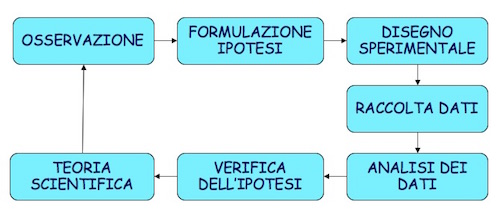
\includegraphics[width=0.75\linewidth]{_images/MSAMap} 

}

\caption{Il metodo scientifico Galileiano}\label{fig:figName11}
\end{figure}

Senza andare troppo in profondità, è importante notare due aspetti:

\begin{enumerate}
\def\labelenumi{\arabic{enumi}.}
\tightlist
\item
  il ruolo fondamentale dell'esperimento scientifico, che produce dati a supporto di ipotesi pre-esistenti;
\item
  lo sviluppo di teorie basate sui dati, che rimangono valide fino a che non si raccolgono altri dati che le confutano, facendo nascere nuove ipotesi che possono portare allo sviluppo di nuove teorie, più affidabili o più semplici.
\end{enumerate}

Insomma, l'ingrediente fondamentale di una prova scientifica è quello di essere supportata dai dati sperimentali: di fatto, non esiste scienza senza dati! Resta famoso l'aforisma ``In God we trust, all the others bring data,'' attribuito all'ingegnere e statistico americano W. Edwards Deming (1900-1993), anche se pare che egli, in realtà, non l'abbia mai pronunciato.

\hypertarget{dati-buoni-e-cattivi}{%
\section{Dati `buoni' e `cattivi'}\label{dati-buoni-e-cattivi}}

Detto che la scienza si basa sui dati, bisogna anche dire che non tutti i dati sono ugualmente `buoni.' Nelle scienze biologiche, così come nelle altre scienze, è importante che i dati siano in grado di cogliere gli effetti che vogliamo studiare, senza introdurre distorsioni.

In agricoltura e nelle altre scienze quantitative abbiamo a che fare con fenomeni `misurabili' e, di conseguenza, i nostri dati consistono di un set di misure di diverso tipo (ci torneremo nel secondo capitolo). L'aspetto più importante è che, per tutta una serie di motivi che dettaglieremo tra poco, le nostre misure non necessariamente riflettono il valore vero della caratteristica misurata nel nostro soggetto. Ciò è noto con il termine di \textbf{errore sperimentale}, che non significa che abbiamo necessariamente fatto qualcosa di sbagliato. Anzi, l'errore sperimentale è considerato una componente inevitabile di ogni esperimento, in grado di proiettare un alea d'incertezza su ogni risultato scientifico.

Ci sono tre fondamentali fonti di errore sperimentale:

\begin{enumerate}
\def\labelenumi{\arabic{enumi}.}
\tightlist
\item
  Errore di misura
\item
  Variabilità dei soggetti sperimentali
\item
  Campionamento
\end{enumerate}

Gli errori di misura sono legati allo strumento e dipendono dall'errata taratura, dall'impiego di un protocollo sbagliato, da inesattezze strumentali, da errori nella trascrizione dei risultati oppure dall'irregolarità dell'oggetto da misurare. Ad esempio, pensate alla misurazione dell'altezza di una pianta di mais: è facile riscontrare difficoltà legate, ad esempio, all'individuazione del punto esatto in cui inizia il culmo e del punto esatto dove termina l'infiorescenza apicale.

A parte gli errori di misura, ci sono anche altre sorgenti di errore meno evidenti e legate al fatto che, nel lavoro sperimentale, siamo di solito interessati non ad un singolo soggetto, ma ad un gruppo più o meno numeroso. Ad esempio, se dobbiamo misurare l'effetto di un erbicida, non possiamo farlo trattando una sola pianta, ma dobbiamo ripetere le misure su un gruppo di piante, il che ci porta ad avere un gruppo di misure, una diversa dall'altra. Quindi, qual è l'effetto dell'erbicida? Il fatto di avere tanti effetti diversi quante sono le piante studiate crea comunque un certo grado di variabilità che non dipende da alcun errore tecnico, ma è una caratteristica intrinseca del fenomeno biologico in studio.

Di per se', la variabilità naturale dei soggetti sperimentali non sarebbe un grosso problema, in quanto potremmo calcolarci l'effetto medio e ritenerci soddisfatti in relazione alle finalità dell'esperimento. Tuttavia sorge un nuovo problema legato al fatto che spesso i soggetti sono così numerosi che non possiamo misurarli tutti e siamo costretti a misurare un campione composto da un ridotto numero di individui. Abbiamo un nuovo elemento di incertezza: come facciamo ad essere sicuri che la media, o qualunque altra statistica, misurata nel nostro campione rifletta la media dell'intera popolazione? Anche se abbiamo fatto del tutto per scegliere un campione rappresentativo, è evidente che il campione perfetto non esiste: cosa potrebbe succedere se prendessimo un altro campione?

\hypertarget{dati-buoni-e-metodi-buoni}{%
\section{Dati `buoni' e metodi `buoni'}\label{dati-buoni-e-metodi-buoni}}

Quindi la ricerca scientifica non è esente da `errori' in senso lato (componenti di incertezza). Tuttavia, gli errori non sono tutti uguali e si dividono in \textbf{sistematici} ed \textbf{accidentali (casuali)}. L'errore sistematico è provocato da difetti intrinseci dello strumento o incapacità peculiari dell'operatore e tende a ripetersi costantemente e con lo stesso segno in misure successive. Un esempio tipico è quello di una bilancia non tarata, che tende ad aggiungere 20 grammi ad ogni misura che effettuiamo. D'altra parte, l'errore accidentale, essendo di natura casuale, tende a ripresentarsi con valori e segni diversi. Di conseguenza, è ragionevole pensare che le repliche, nel lungo periodo, producano sovrastime e sottostime con uguale probabilità, in modo che la media tende a coincidere con il valore vero.

È facile capire che le conseguenze degli errori sistematici e accidentali sono ben diverse. A questi proposito, dobbiamo considerare due aspetti molto importanti, cioè:

\begin{enumerate}
\def\labelenumi{\arabic{enumi}.}
\tightlist
\item
  precisione
\item
  accuratezza
\end{enumerate}

Con il termine \textbf{precisione} intendiamo due cose: la prima è relativa al numero di decimali che ci fornisce il nostro strumento di misura. E'evidente, ad esempio, come un calibro sia più preciso di un metro da sarto. Oltre a questo significato, abbastanza intuitivo, ce n'è un altro, più specificatamente legato agli esperimenti scientifici: la precisione di un dato ottenuto attraverso un processo di misurazione non è altro che la variabilità riscontrata quando la misurazione viene ripetuta più volte. L'errore casuale produce sempre un calo di precisione.

Il termine accuratezza ha invece un significato completamente diverso, riconducibile alla differenza tra la misura effettuata e il valore vero della caratteristica da misurare. Può sembrare una banalità, ma proviamo a pensare ad uno strumento non tarato, come, ad esempio, un gascromatografo, che restituisce sempre una concentrazione maggiorata del 20\%. Se noi ripetessimo le analisi 100 volte, in assenza di altri errori, otterremmo sempre lo stesso risultato, molto preciso, ma totalmente inaffidabile, nel senso che non riflette la concentrazione reale della soluzione in studio. L'errore sistematico, oltre a produrre un calo di precisione, produce anche inaccuratezza.

Comprendiamo bene che l'accuratezza è più importante della precisione: infatti una misura accurata, ma imprecisa, riflette bene la realtà, anche se in modo vago. Al contrario, una misura precisa, ma inaccurata, ci porta completamente fuori strada, perché non riflette la realtà. Con linguaggio tecnico, un dato non accurato si dice `distorto' (\emph{biased}) e, siccome la distosione dipende dagli errori sistematici, questi ultimi vanno assolutamente evitati, ad esempio con la perfetta taratura degli strumenti e l'adozione di metodi di misura rigidamente standardizzati e accettati dalla comunità scientifica mondiale.

L'inaccuratezza preoccupa molto i laboratori di analisi, che spesso utilizzano standard di confronto, la cui misura è perfettamente nota e viene periodicamente confrontata con quella rilevabile dallo strumento stesso, per verificarne la taratura. Altro metodo utilizzato nelle procedure di accreditamento dei laboratori è il \emph{ring test}, dove campioni reali della matrice da misurare sono inviati a più laboratori a livello nazionale, in modo da poter confrontare le misure ottenute e valutarne la variabilità. Con un \emph{ring test}, un laboratorio può valutare la sua stessa affidabilità in confronto con laboratori simili, basandosi sull'eventuale differenza tra il risultato ottenuto e quelli ottenuti in tutti gli altri laboratori valutati.

Sfortunatamente la possibilità di raccogliere dati inaccurati è tutt'altro che remota. Gli scienziati americani Pons e Fleischmann, il 23 Marzo del 1989, diffusero pubblicamente la notizia di essere riusciti a riprodurre la fusione nucleare fredda, causando elevatissimo interesse nella comunità scientifica. Purtroppo le loro misure erano viziate da una serie di problemi e il loro risultato fu smentito da esperimenti successivi.

\begin{figure}

{\centering 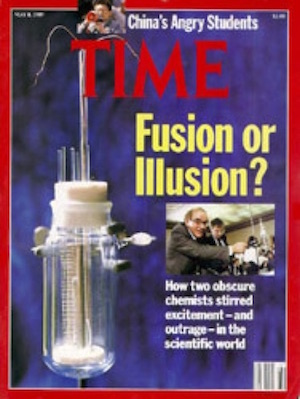
\includegraphics[width=0.5\linewidth]{_images/FalseResults} 

}

\caption{Conseguenze di un esperimento sbagliato}\label{fig:figName2}
\end{figure}

A parte questo clamoroso esempio, torniamo alla nostra domanda iniziale: come facciamo ad essere sicuri che i dati siano validi ed affidabili? La risposta è semplice: non possiamo mai essere sicuri, ma \textbf{dobbiamo fare del nostro meglio per applicare metodi rigorosi, così da minimizzare la possibilità di ottenere errori sistematici}. In altre parole, dati `buoni' sono conseguenza di metodi `buoni' e, pertanto \textbf{una prova scientifica è tale non perché siamo certi che corrisponda alla realtà, ma perché siamo ragionevolmente certi che sia stata ottenuta con metodi validi!}.

\hypertarget{il-principio-di-falsificazione}{%
\section{Il principio di falsificazione}\label{il-principio-di-falsificazione}}

L'approccio che abbiamo indicato poco sopra ha un'importante conseguenza: anche se abbiamo utilizzato un metodo perfettamente valido non potremo mai avere la certezza di aver ottenuto un risultato corrispondente alla realtà e, quindi, ci dovremo sempre aspettare che ulteriori dati smentiscano la nostra conclusione. Questa è la base del principio di falsificazione, definito da Karl Popper (1902-1994): non potremo mai dimostrare che una nostra ipotesi è vera, ma potremo solo dimostrare che è falsa.

In pratica, tornando al metodo scientifico, partiamo da un'ipotesi e organizziamo un esperimento perfettamente valido che produce, di conseguenza, dati validi. Se i nostri dati sconfermano l'ipotesi, abbiamo dimostrato che questa è falsa e dovremo quindi produrre una nuova ipotesi da sottoporre a verifica. Se invece i dati confermano la nostra ipotesi (o meglio, non la smentiscono) allora, non potremo concludere che l'ipotesi è vera, in quanto rimarrà sempre il dubbio che non abbiamo raccolto abbastanza dati. Tuttavia, in mancanza di altre informazioni, prenderemo per buona la nostra ipotesi, fino a che non sarà smentita. Una sorta di `assoluzione' per insufficienza di prove, quindi\ldots{}

Il principio di falsificazione è piuttosto importante nel mondo scientifico ed ha alcune importanti implicazioni:

\begin{enumerate}
\def\labelenumi{\arabic{enumi}.}
\tightlist
\item
  Scienza non necessariamente significa `certezza' o `verità.' Tutto quello che possiamo fare con certezza è rigettare ipotesi (provare che sono false), ma non dimostrarne la validità.
\item
  Il nostro compito è quello di cercare di eliminare tutte le fonti di errore sistematico, per rendere il risultato il più accurato possibile.
\item
  Eliminato l'errore sistematico, l'evantuale errore casuale residuo deve essere sempre quantificato e visualizzato insieme ai risultati.
\item
  In considerazione dell'errore residuo, dobbiamo decidere se i dati raccolti consentono di rigettare la nostra ipotesi di partenza. Altrimenti, l'esperimento è inconclusivo e, pur non avendone la certezza, terremo per vera la nostra ipotesi di partenza fino a che non sarà smentita da future osservazioni.
\end{enumerate}

Oltre al principio di falsificazione, la scienza fa largo uso del principio del `rasoio di Occam.' Guglielmo di Occam (XIV secolo) era un frate francescano che, in un periodo in cui le dimostrazioni scientifiche iniziavano a divenire troppo complesse, voleva ribadire l'importanza della semplicità. Il suo principio è solitamente formulato come `\emph{Entia non sunt multiplicanda praeter necessitatem}' ed è noto come il `rasoio' in quanto porta a respingere con nettezza (tagliare con il rasoio) le spiegazioni troppo complesse. Nella comunità scientifica, applichiamo questo principio preferendo sempre, tra due ipotesi alternative ugualmente buone, quella più semplice.

\hypertarget{falsificare-un-risultato}{%
\section{Falsificare un risultato}\label{falsificare-un-risultato}}

Se un esperimento è inconclusivo e porta ad eccettare un'ipotesi, è sempre possibile eseguire un ulteriore esperimento per rigettarla. Se anche questo secondo esperimento non riesce a rigettare l'ipotesi di partenza, allora la bontà di quest'ultima è certamente rafforzata. Parliamo quindi di esperimenti confermativi che costituiscono un elemento molto importante del metodo scientifico.

A questo proposito, distinguiamo:

\begin{enumerate}
\def\labelenumi{\arabic{enumi}.}
\tightlist
\item
  replicabilità
\item
  riproducibilità
\end{enumerate}

Un esperimento è replicabile se, quando ripetuto in condizioni assolutamente analoghe (stessi soggetti, ambiente, strumenti\ldots), restituisce risultati equivalenti. Per questo motivo, quando si pubblicano i risultati di un esperimento, è sempre necessario descrivere accuratamente i metodi impiegati, in modo da consentire a chiunque la verifica dei risultati.

In alcuni casi, tuttavia, questa verifica indipendente è pressoché impossibile; ad esempio, nelle scienze agronomiche, le caratteristiche genetiche e pedo-climatiche giocano un ruolo molto importante e non è facile replicare un esperimento di pieno campo esattamente nelle stesse condizioni. Per questo motivo, alcuni biostatistici distinguono la replicabilità dalla riproducibilità, definita come il grado di concordanza tra esperimenti ripetuti in condizioni diverse (diversi soggetti, diverso ambiente\ldots). Se la replicabilità di un esperimento non può essere dimostrata, bisogna avere almeno un'idea della sua riproducibilità, ripetendo l'esperimento in condizioni diverse e discutendo attentamente le eventuali differenze riscontrate nei risultati.

\begin{center}\rule{0.5\linewidth}{0.5pt}\end{center}

\hypertarget{elementi-fondamentali-del-disegno-sperimentale}{%
\section{Elementi fondamentali del disegno sperimentale}\label{elementi-fondamentali-del-disegno-sperimentale}}

La metodica di organizzazione di un esperimento valido prende il nome di \emph{disegno sperimentale} e le sue basi si fanno in genere risalire a Sir Ronald A. Fisher, vissuto in Inghilterra dal 7 Febbraio 1890 al 29 luglio 1962. Laureatosi nel 1912, lavora come statistico per il comune di Londra, fino a quando diviene socio della prestigiosa Eugenics Education Society di Cambridge, fondata nel 1909 da Francis Galton, cugino di Charles Darwin. Dopo la fine della guerra, Karl Pearson gli propone un lavoro presso il rinomato Galton Laboratory, ma egli non accetta a causa della profonda rivalità esistente tra lui e Pearson stesso. Nel 1919 viene assunto presso la Rothamsted Experimental Station, dove si occupa dell'elaborazione dei dati sperimentali e, nel corso dei successivi 7 anni, definisce le basi del disegno sperimentale ed elabora la sua teoria della ``analysis of variance.'' Il suo libro più importante è ``The design of experiment,'' del 1935. E' sua la definizione delle tre componenti fondamentali del disegno sperimentale:

\begin{enumerate}
\def\labelenumi{\arabic{enumi}.}
\tightlist
\item
  controllo degli errori;
\item
  replicazione;
\item
  randomizzazione.
\end{enumerate}

\hypertarget{controllo-degli-errori}{%
\subsection{Controllo degli errori}\label{controllo-degli-errori}}

Controllare gli errori, o, analogamente, eseguire un esperimento controllato significa fondamentalmente due cose:

\begin{enumerate}
\def\labelenumi{\arabic{enumi}.}
\tightlist
\item
  adottare provvedimenti idonei ad evitare le fonti di errore, mantenendole al livello più basso possibile (alta precisione);
\item
  agire in modo da isolare l'effetto in studio (accuratezza), evitando che si confonda con effetti casuali e di altra natura. Ad esempio, se dobbiamo confrontare due fitofarmaci, dobbiamo fare in modo che i soggetti inclusi nell'esperimento differiscano tra di loro solo per il fitofarmaco impiegato e non per altro.
\end{enumerate}

Mettere in pratica questi principi fondamentali richiede una vita di esperienza! Tuttavia, vogliamo solo sottolineare alcuni aspetti, come il rigore metodologico. È evidente che, ad esempio, se vogliamo sapere la cinetica di degradazione di un erbicida a 20 °C dovremo realizzare una prova esattamente a quella temperatura, con un erbicida uniformemente distribuito nel terreno, dentro una camera climatica capace di un controllo perfetto della temperatura. Gli strumenti dovranno essere ben tarati e sarà necessario attenersi scrupolosamente a metodi validati e largamente condivisi. Tuttavia, a proposito di rigore, non bisogna scordare quanto diceva C.F. Gauss a proposito della precisione nei calcoli, e che può essere anche riferito al rigore nella ricerca : ``\emph{Manca di mentalità matematica tanto chi non sa riconoscere rapidamente ciò che è evidente, quanto chi si attarda nei calcoli con una precisione superiore alla necessità}''

Oltre al rigore metodologico, è bene anche ricordare come un esperimento ben fatto passi sempre attraverso la giusta selezione dei soggetti sperimentali, che debbono essere omogenei, ma rappresentativi della popolazione alla quale intendiamo riferire i risultati ottenuti. Ad esempio, se si vuole ottenere un risultato riferito alla collina umbra, bisognerà scegliere parcelle di terreno omogenee, ma che rappresentano bene la variabilità pedo-climatica di quell'ambiente, né di più, né di meno.

Per concludere, vogliamo anche ricordare le cosiddette `intrusioni' cioè quegli eventi che accadono in modo inaspettato e condizionano negativamente la riuscita di un esperimento in corso. E' evidente che, ad esempio, un'alluvione, l'attacco di insetti o patogeni, la carenza idrica hanno una pesante ricaduta sulla precisione di un esperimento e sulla sua riuscita. Per quanto possibile, controllare gli errori significa anche essere capaci di prevedere le eventuali intrusioni. In un suo famoso lavoro scientifico del 1984, lo scienziato americano Stuart Hurlbert usa il termine `intrusione demoniaca' per indicare quelle intrusioni che, pur casuali, avrebbero potuto essere previste con un disegno più accurato, sottolineando in questo caso la responsabilità dello sperimentatore.

Un esempio è questo: uno sperimentatore vuole studiare l'entità della predazione dovuta alle volpi e quindi usa campi senza staccionate (dove le volpi possono entrare) e campi protetti da staccionate (e quindi liberi da volpi). Se le staccionate, essendo utilizzate dai falchi come punto d'appoggio, finiscono per incrementare l'attività predatoria di questi ultimi, si viene a creare un'intrusione demoniaca, che rende l'esperimento distorto. Il demonio, in questo caso, non è il falco, che danneggia l'esperimento, ma il ricercatore stesso, che non ha saputo prevedere una possibile intrusione.

\hypertarget{replicazione}{%
\subsection{Replicazione}\label{replicazione}}

In ogni esperimento, i trattamenti dovrebbe essere replicati su due o più unità sperimentali. Ciò permette di:

\begin{enumerate}
\def\labelenumi{\arabic{enumi}.}
\tightlist
\item
  dimostrare che i risultati sono replicabili (ma non è detto che siano riproducibili!);
\item
  rassicurare che eventuali circostanze aberranti casuali non abbiano provocato risultati distorti;
\item
  misurare la precisione dell'esperimento, come variabilità di risposta tra repliche trattate nello stesso modo;
\item
  incrementare la precisione dell'esperimento (più sono le repliche più l'esperimento è preciso, perché si migliora la stima della caratteristica misurata, diminuendo l'incertezza).
\end{enumerate}

Per poter essere utili, le repliche debbono essere indipendenti, cioè debbono \textbf{aver subito tutte le manipolazioni necessarie per l'allocazione del trattamento in modo totalmente indipendente l'una dall'altra}. Le manipolazioni comprendono tutte le pratiche necessarie, come ad esempio la preparazione delle soluzioni, la diluizione dei prodotti, ecc..

La manipolazione indipendente è fondamentale, perché in ogni parte del processo di trattamento possono nascondersi errori più o meno grandi, che possono essere riconosciuti solo se colpiscono in modo casuale le unità sperimentali. Se la manipolazione è, anche solo in parte, comune, questi errori colpiscono tutte le repliche allo stesso modo, diventano sistematici e quindi non più riconoscibili. Di conseguenza, si inficia l'accuratezza dell'esperimento. Quando le repliche non sono indipendenti, si parla di \textbf{pseudorepliche}, contrapposte alle \textbf{repliche vere}.

Il numero di repliche dipende dal tipo di esperimento: più sono e meglio è, anche se è necessario trovare un equilibrio accettabile tra precisione e costo dell'esperimento. Nella sperimentazione di campo, due repliche sono poche, tre appena sufficienti, quattro costituiscono la situazione più comune, mentre un numero maggiore di repliche è abbastanza raro, non solo per la difficoltà di seguire l'esperimento, ma anche perché aumentano la dimensione della prova e, di conseguenza, la variabilità del terreno.

\hypertarget{randomizzazione}{%
\subsection{Randomizzazione}\label{randomizzazione}}

L'indipendenza di manipolazione non garantisce da sola un esperimento corretto. Infatti potrebbe accadere che le caratteristiche innate dei soggetti, o una qualche `intrusione' influenzino in modo sistematico tutte le unità sperimentali trattate nello stesso modo, così da confondersi con l'effetto del trattamento. Un esempio banale è che potremmo somministrare un farmaco a quattro soggetti in modo totalmente indipendente, ma se i quattro soggetti fossero sistematicamente più alti di quelli non trattati finiremmo per confondere una caratteristica innata con l'effetto del farmaco. Oppure, se le piante di una certa varietà di sorgo si trovassero tutte più vicine alla scolina rispetto a quelle di un'altra varietà, potrebbero essere più danneggiate dal ristagno idrico, il cui effetto si confonderebbe con quello del trattamento stesso.

Questi problemi sono particolarmente insidiosi e si nascondono anche dietro ai particolari apparentemente più insignificanti. La randomizzazione è l'unico sistema per evitare, o almeno rendere molto improbabile, la confusione dell'effetto del trattamento con fattori casuali e/o comunque diversi dal trattamento stesso. La randomizzazione si declina in vari modi:

\begin{enumerate}
\def\labelenumi{\arabic{enumi}.}
\tightlist
\item
  allocazione casuale del trattamento alle unità sperimentali. Gli esperimenti che prevedono l'allocazione del trattamento sono detti `manipolativi' o `disegnati.'
\item
  A volte l'allocazione del trattamento non è possibile o non è etica. Se volessimo studiare l'effetto delle cinture di sicurezza nell'evitare infortuni gravi, non potremmo certamente provocare incidenti deliberati. In questo caso la randomizzazione è legata alla scelta casuale di soggetti che sono `naturalmente' trattati. Esperimenti di questi tipo, si dicono \textbf{osservazionali}. Un esempio è la valutazione dell'effetto dell'inquinamento con metalli pesanti nella salute degli animali: ovviamente non è possibile, se non su piccola scala, realizzare il livello di inquinamento desiderato e, pertanto, dovremo scegliere soggetti che sono naturalmente sottoposti a questo genere di inquinamento, magari perché vivono vicino a zone industriali.
\item
  Se i soggetti sono immobili, la randomizzazione ha anche una connotazione legata alla disposizione spaziale e/o temporale casuale.
\end{enumerate}

L'assegnazione casuale del trattamento, o la selezione casuale dei soggetti trattati, fanno si che tutti i soggetti abbiano la stessa probabilità di ricevere qualunque trattamento oppure qualunque intrusione casuale. In questo modo, la probabilità che tutte le repliche di un trattamento abbiano qualche caratteristica innata o qualche intrusione comune che li penalizzi/avvantaggi viene minimizzata. Di conseguenza, confondere l'effetto del trattamento con variabilità casuale (`confounding'), anche se teoricamente possibile, diviene altamente improbabile.

\hypertarget{esperimenti-invalidi}{%
\subsection{Esperimenti invalidi}\label{esperimenti-invalidi}}

A questo punto, dovrebbe essere chiaro che un esperimento valido deve essere controllato, replicato e randomizzato: la mancanza anche di uno solo di questi elementi pone dubbi ragionevoli sull'affidabilità dei risultati. In particolare, gli esperimenti `invalidi' sono caratterizzati da:

\begin{enumerate}
\def\labelenumi{\arabic{enumi}.}
\tightlist
\item
  Cattivo controllo degli errori
\item
  Fondati sospetti di confounding
\item
  Mancanza di repliche vere
\item
  Confusione tra repliche vere e pseudo-repliche
\item
  Mancanza di randomizzazione
\item
  Presenza di vincoli alla randomizzazione, trascurati in fase di analisi.
\end{enumerate}

Le conseguenze di queste problematiche sono abbastanza diverse.

\hypertarget{cattivo-controllo-degli-errori}{%
\subsubsection{Cattivo controllo degli errori}\label{cattivo-controllo-degli-errori}}

Bisogna verificare se il problema è relativo a questioni come la mancanza di scrupolosità, l'uso di soggetti poco omogenei o di un ambiente poco omogeneo, o altri aspetti che inficiano solo la precisione, ma non l'accuratezza dell'esperimento. In questo caso, l'esperimento è ancora valido (accurato), ma la bassa precisione probabilmente impedirà di trarre conclusioni forti. Quindi, un esperimento impreciso si `elimina' da solo, perché sarà inconclusivo. Di questi esperimenti bisogna comunque diffidare, soprattutto quando siano pianificati per mostrare l'assenza di differenze tra due trattamenti alternativi. Mostrare l'assenza di differenze è facile: basta fare male un esperimento, in modo che vi sia un alto livello di incertezza e quindi l'evidenza scientifica sia molto debole.

Diversa è la situazione in cui un cattivo controllo degli errori, ad esempio l'adozione di metodi sbagliati, porta a mancanza di accuratezza, cioè a risultati che non riflettono la realtà (campionamento sbagliato, ad esempio; oppure strumenti non tarati; impiego di metodi non validati e/o non accettabili). In questo caso venendo a mancare l'accuratezza, l'esperimento deve essere rigettato, in quanto non fornisce informazioni realistiche.

\hypertarget{confounding-e-correlazione-spuria}{%
\subsubsection{`Confounding' e correlazione spuria}\label{confounding-e-correlazione-spuria}}

Abbiamo appena menzionato il problema fondamentale della ricerca, cioè il \textbf{confounding}, vale a dire la confusione tra l'effetto del trattamento e un qualche altro effetto casuale, legato alle caratteristiche innate del soggetto o a qualche intrusione più o meno `demoniaca.' Abbiamo detto che non possiamo mai avere la certezza dell'assenza di confounding, ma abbiamo anche detto che l'adozione di una pratica sperimentale corretta ne minimizza la probabilità.

Chiaramente, rimangono dei rischi che sono tipici di situazioni nelle quali il controllo adottato non è perfetto, come capita, ad esempio, negli esperimenti osservazionali. In questo ambito è piuttosto temuta la cosiddetta `correlazione spuria,' una forma di confounding casuale per cui due variabili variano congiuntamente (sono direttamente o inversamente proporzionali), ma in modo del tutto casuale. Esistono, ad esempio, dati che mostrano una chiara correlazione tra le vendite di panna acida e le morti per incidenti in motocicletta (Figura 1.3). Chiaramente, non esistono spiegazioni scientifiche per questo effetto, che è, ovviamente, del tutto casuale. Il problema è che questa correlazione spuria non è sempre così semplice da rintracciare.

\begin{figure}

{\centering 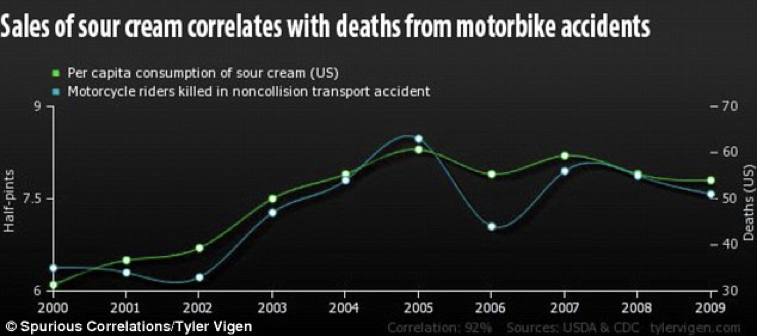
\includegraphics[width=0.9\linewidth]{_images/PannaAcida} 

}

\caption{Esempio di correlazione spuria}\label{fig:figName22}
\end{figure}

A volte il confounding non è casuale, ma è legato ad una variabile esterna che si agisce all'insaputa dello sperimentatore. Ad esempio, è stato osservato che il tasso di crimini è più alto nelle città che hanno più chiese. La spiegazione di questo paradosso sta nel fatto che esiste un `confounder,' cioè l'ampiezza della popolazione. Nelle grandi città si riscontrano sia una maggiore incidenza criminale, sia un grande numero di chiese. In sostanza, la popolazione determina sia l'elevato numero di chiese che l'elevato numero di crimini, ma queste ultime due variabili non sono legate tra loro da una relazione causa-effetto (A implica B e A implica C, ma B non implica C).

Il confounding non casuale è spesso difficile da evidenziare, soprattutto se le correlazioni misurate sono spiegabili. Inoltre, non è eliminabile con un'accurata randomizzazione, ma solo con l'esecuzione di un esperimento totalmente controllato, nel quale ci si preoccupa di rilevare tutte le variabili necessarie per spiegare gli effetti riscontrati. Di questo è importante tener conto soprattutto negli esperimenti osservazionali, dove il controllo è sempre più difficile e meno completo.

\hypertarget{pseudo-repliche-e-randomizzazione-poco-attenta}{%
\subsubsection{Pseudo-repliche e randomizzazione poco attenta}\label{pseudo-repliche-e-randomizzazione-poco-attenta}}

Per evidenziare questi problemi e comprendere meglio la differenza tra un esperimento corretto e uno non corretto, è utilissima la classificazione fatta da Hurlbert (1984), che riportiamo di seguito.

\begin{figure}

{\centering 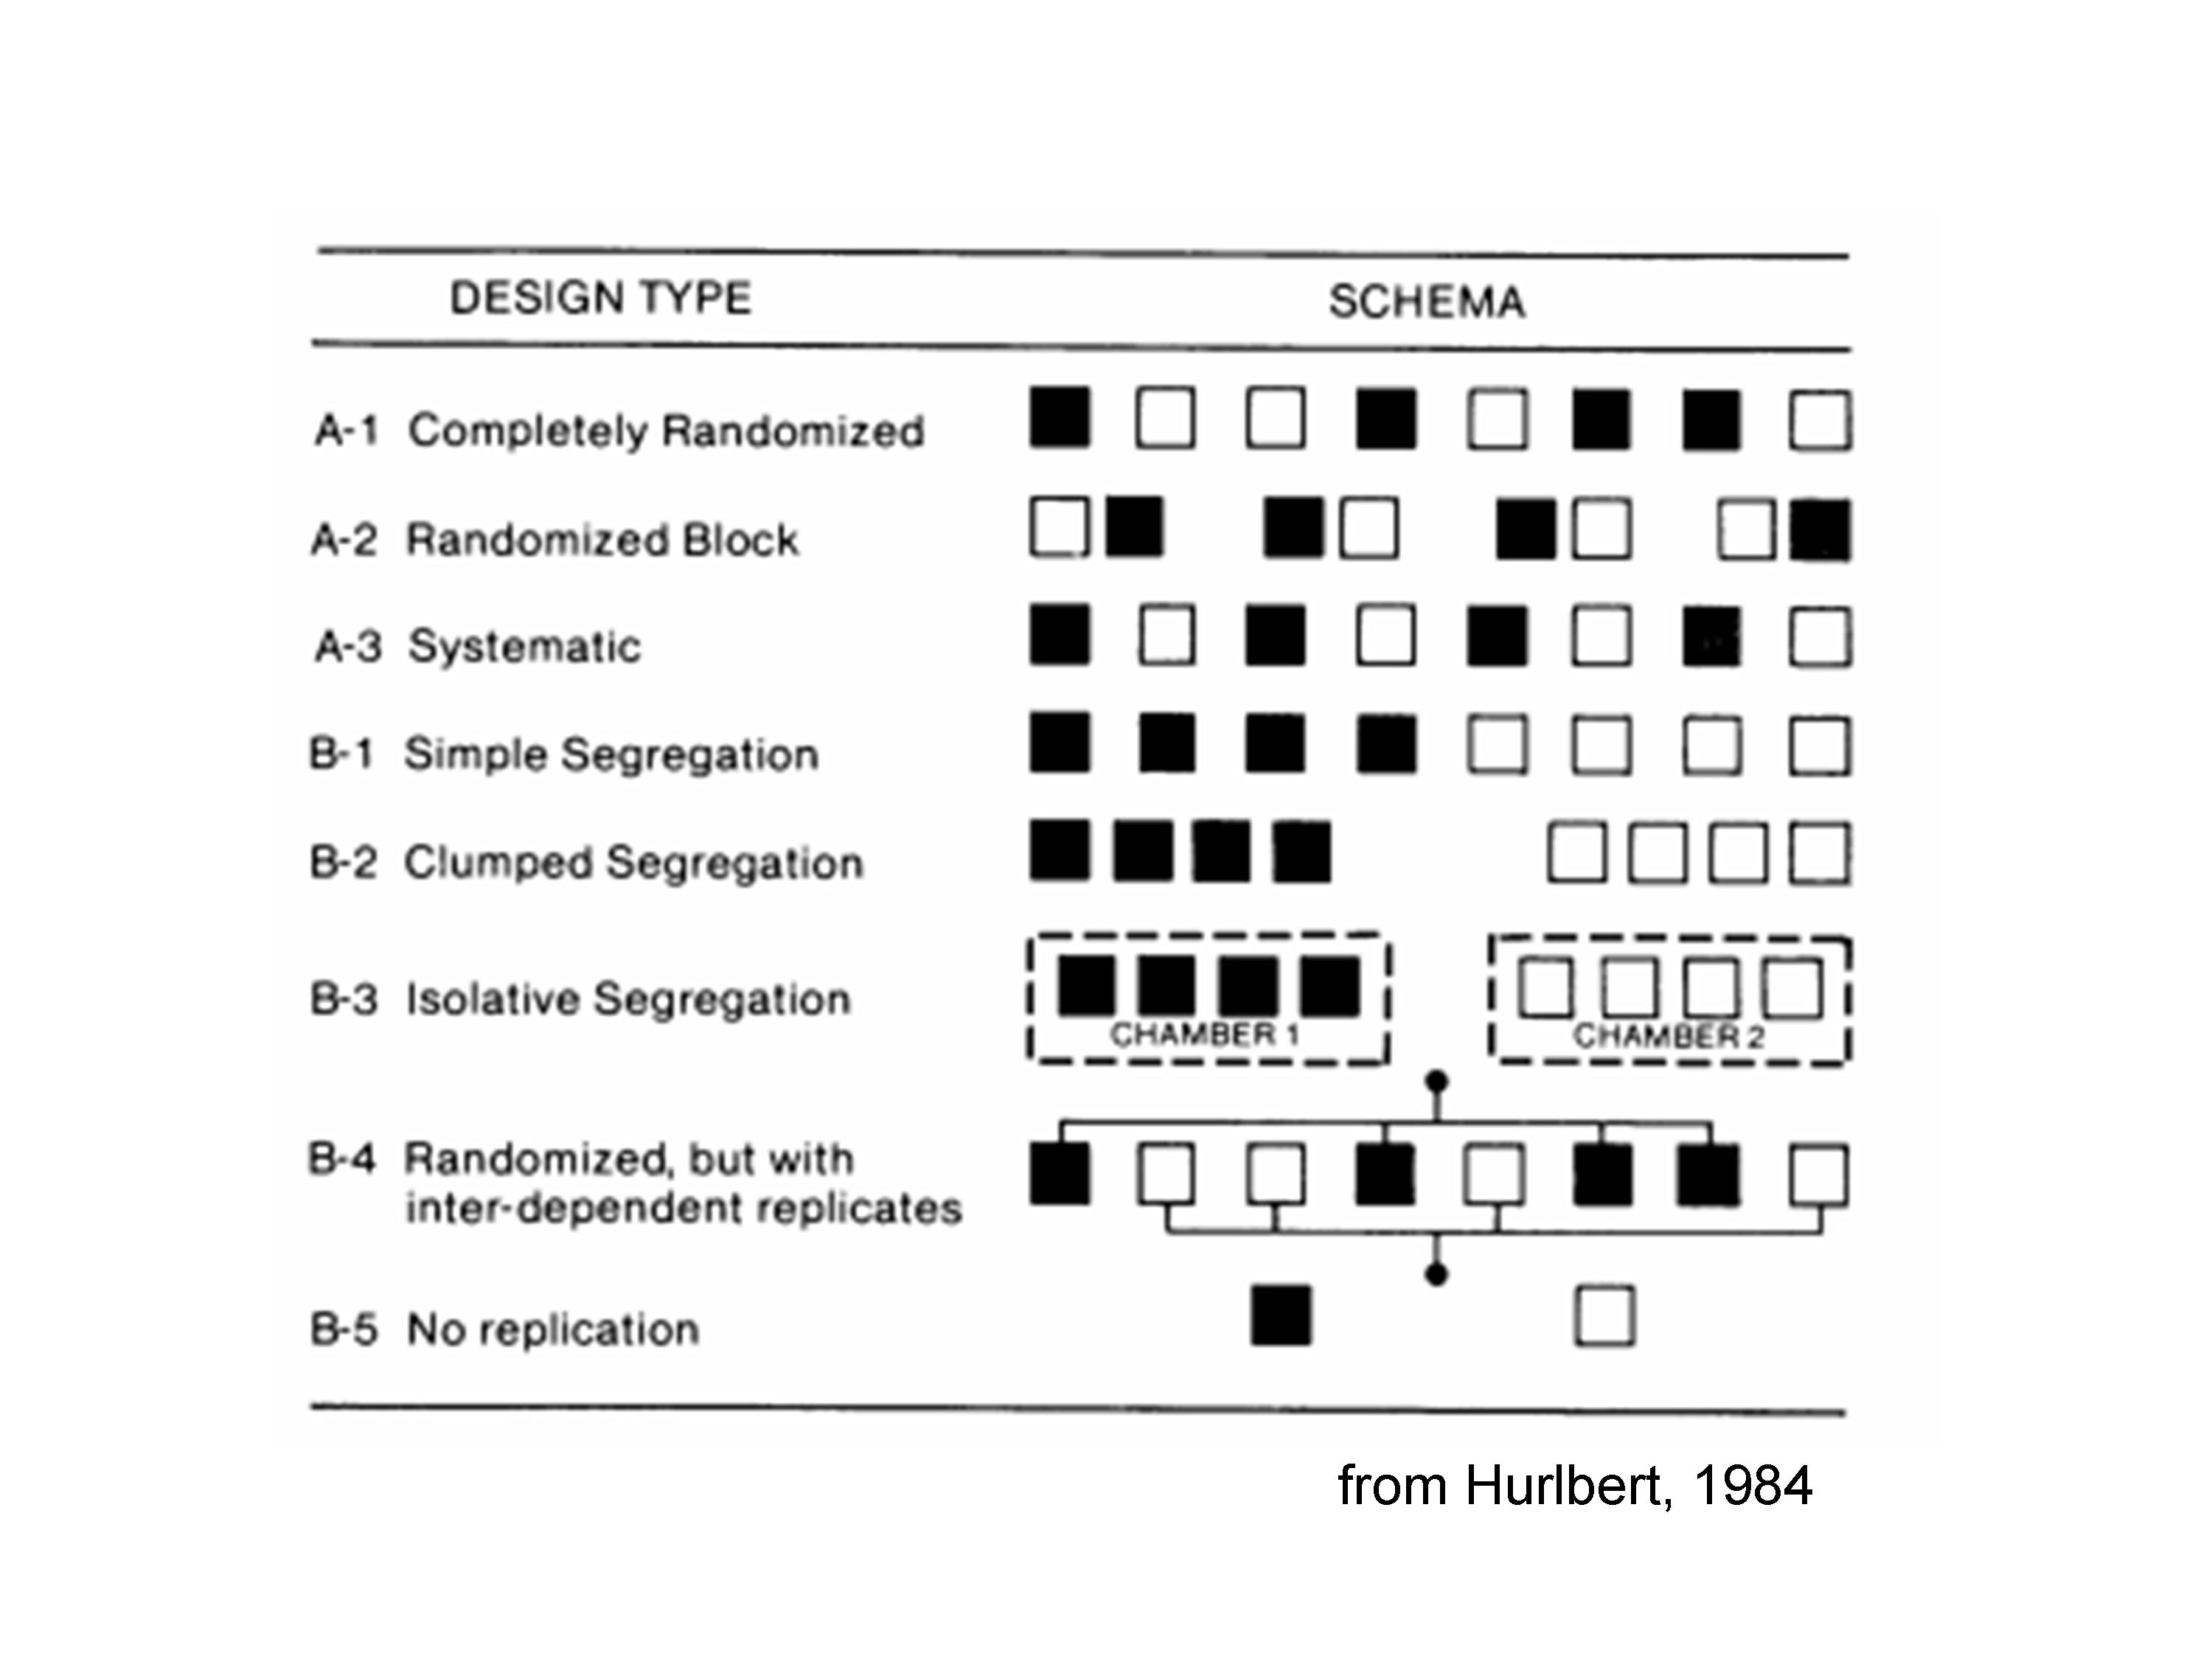
\includegraphics[width=0.9\linewidth]{_images/Randomisation} 

}

\caption{Indicazioni per una corretta randomizzazione (Hurlbert, 1984)}\label{fig:figName23}
\end{figure}

Vengono mostrati 8 soggetti, sottoposti a due trattamenti (bianco e nero), con 8 disegni sperimentali diversi.

Il disegno A1 è corretto, in quanto si tratta di un esperimento completamente randomizzato. Ugualmente, è valido il disegno A2, nel quale le unità sperimentali sono state divise in quattro gruppi omogenei e sono state trattate in modo randomizzato all'interno di ogni gruppo.

Il disegno A3 è quantomeno `sospetto': vi sono repliche vere, ma l'allocazione dei trattamenti non è randomizzata ed avviene con un processo sistematico per il quale `nero' e `bianco' si alternano. Cosa succederebbe se vi fosse un gradiente di fertilità decrescente da destra verso sinistra? Le unità nere sarebbero avvantaggiate rispetto alle bianche! Insomma, rimangono sospetti di confounding, a meno che non si sia assolutamente certi dell'assenza di gradienti, come capita ad esempio se all'interno dei blocchi, dobbiamo creare una sequenza spazio-temporale. Vediamo tre esempi:

\begin{enumerate}
\def\labelenumi{\arabic{enumi}.}
\tightlist
\item
  ho quattro piante e, per ogni pianta, voglio confrontare un ramo basso con uno alto: è evidente che i due trattamenti sono sempre ordinati in modo sistematico (basso prima di alto).
\item
  Dobbiamo valutare l'effetto di fitofarmaci somministrati in due epoche diverse (accestimento e inizio-levata); anche qui non possiamo randomizzare, giacché un'epoca precede sempre l'altra.
\item
  Dobbiamo confrontare la presenza di residui di un fitofarmaco a due profondità e non possiamo randomizzare, perché una profondità precede sempre l'altra nello spazio.
\end{enumerate}

In queste situazioni l'esperimento rimane valido, anche se la randomizzazione segue un processo sistematico e non casuale.

Il disegno B1 è usualmente invalido: non vi è randomizzazione e ciò massimizza i problemi del disegno A3: la separazione delle unità sperimentali `bianche' e `nere' non consente una valutazione adeguata dell'effetto del trattamento, che è confuso con ogni potenziale differenza tra la parte destra e la sinistra dell'ambiente in cui la sperimentazione viene eseguita. Ovviamente, la separazione può essere non solo spaziale, ma anche temporale. Anche in questo caso diamo alcuni esempi in cui una situazione come quella descritta in B1 è valida:

\begin{enumerate}
\def\labelenumi{\arabic{enumi}.}
\tightlist
\item
  Vogliamo confrontare la produzione in pianura e in collina. Ovviamente dobbiamo scegliere campioni in due situazioni fisicamente separate
\item
  Vogliamo confrontare la pescosità di due laghetti
\item
  Vogliamo confrontare la produttività di due campi contigui.
\end{enumerate}

Queste situazioni sono valide, anche se con una restrizione: non siamo in grado di stabilire a chi debba essere attribuito l'effetto. Ad esempio, per la prima situazione, pianura e collina possono dare produzioni diverse per il suolo diverso, il clima diverso, la precessione colturale diversa o un qualunque altro elemento che differenzi le due località.

Il disegno B2 è analogo al disegno B1, ma il problema è più grave, perché la separazione fisica è più evidente. Questo disegno è totalmente sbagliato, a meno che non siamo specificatamente interessati all'effetto località (vedi sopra).

Il disegno B3 è analogo al disegno B2, ma costituisce una situazione molto frequente nella pratica scientifica. Immaginiamo infatti di voler confrontare la germinazione dei semi a due temperature diverse, utilizzando due camere climatiche e mettendo, in ognuna di esse, quattro capsule Petri identiche. In questa situazione, l'effetto temperatura è totalmente confuso con l'effetto `camera climatica (località)' e risente di ogni malfunzionamento relativo ad una sola delle due camere. Inoltre, le unità sperimentali con lo stesso trattamento di temperature non sono manipolate in modo indipendente, dato che condividono la stessa camera climatica. Di conseguenza, non si può parlare di repliche vere, bensì di \textbf{pseudorepliche}.

Altri esempi di \textbf{pseudorepliche} sono schematizzati con il codice B4. Ad esempio:

\begin{enumerate}
\def\labelenumi{\arabic{enumi}.}
\tightlist
\item
  trattare piante in vaso ed analizzare in modo indipendente i singoli individui invece che tutto il vaso;
\item
  trattare una parcella di terreno e prelevare da essa più campioni, analizzandoli separatamente;
\item
  trattare una capsula Petri ed analizzare separatamente i semi germinati al suo interno.
\end{enumerate}

Questi disegni, in assenza di repliche vere aggiuntive non sono da considerarsi validi. Ad esempio, se io ho due vasetti trattati in modo totalmente indipendente e da ciascuno di essi prelevo due piante e le analizzo separatamente, il disegno è caratterizzato da due repliche vere e due pseudorepliche per ogni replica ed è, pertanto, valido.

Il disegno B5 è invece evidentemente invalido, per totale mancanza di repliche.

\hypertarget{chi-valuta-se-un-esperimento-uxe8-attendibile}{%
\section{Chi valuta se un esperimento è attendibile?}\label{chi-valuta-se-un-esperimento-uxe8-attendibile}}

Quanto detto finora vorrebbe chiarire come il punto centrale della scienza non è la certezza delle teorie, bensì il metodo che viene utilizzato per definirle. Ognuno di noi è quindi responsabile di verificare che le informazioni in suo possesso siano `scientificamente' attendibili, cioè ottenute con un metodo sperimentale adeguato. Il fatto è che non sempre siamo in grado di compiere questa verifica, perché non abbiamo strumenti `culturali' adeguati, se non nel ristretto ambito delle nostre competenze professionali. Come fare allora?

L'unica risposta accettabile è quella di controllare l'attendibilità delle fonti di informazione. In ambito biologico, le riviste autorevoli sono caratterizzate dal procedimento di `\emph{peer review},' nel quale i manoscritti scientifici, prima della pubblicazione, sono sottoposti ad un comitato editoriale ed assegnati ad un `editor,' il quale legge il lavoro e contemporaneamente lo invia a due o tre scienziati anonimi e particolarmente competenti in quello specifico settore scientifico (\emph{reviewers} o revisori).

I revisori, insieme all'\emph{editor}, compiono un attento lavoro di esame e stabiliscono se l'evidenza scientifica presentata è sufficientemente `forte.' Le eventuali critiche vengono presentate all'autore, che è tenuto a rispondere in modo convincente, anche ripetendo gli esperimenti se necessario. Il processo richiede spesso interi mesi ed è abbastanza impegnativo per uno scenziato. E' piuttosto significativa l'immagine presentata in \href{http://scienceblogs.com/startswithabang/2013/06/07/the-4-jobs-of-a-referee-in-peer-review/}{scienceBlog.com}, che allego qui.

\begin{figure}

{\centering 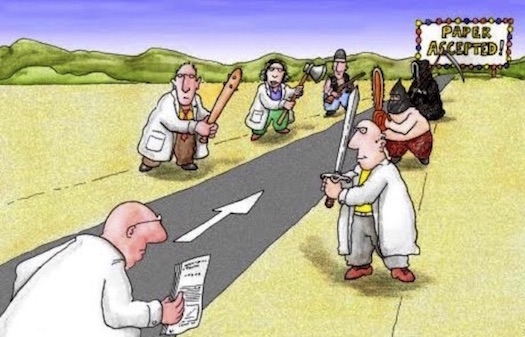
\includegraphics[width=0.75\linewidth]{_images/PeerReview} 

}

\caption{Il processo di peer review}\label{fig:figName3}
\end{figure}

In sostanza il meccanismo di \emph{peer review} porta a rigettare un lavoro scientifico in presenza di qualunque ragionevole dubbio metodologico. Desideriamo sottolineare che abbiamo parlato di dubbio metodologico, dato che il dubbio sul risultato non può essere allontanato completamente e i reviewer controlleranno solo che il rischio di errore sia al disotto della soglia massima arbitrariamente stabilita (di solito pari al 5\%). Questo procedimento, se effettuato con competenza, dovrebbe aiutare a separare la scienza dalla pseudo-scienza e, comunque, ad eliminare la gran parte degli errori metodologici dai lavori scientifici.

\hypertarget{conclusioni}{%
\section{Conclusioni}\label{conclusioni}}

In conclusione, possiamo ripartire dalla domanda iniziale: ``Che cosa è la scienza?'' per rispondere che è scienza tutto ciò che è supportato da dati che abbiano passato il vaglio della \emph{peer review}, dimostrando di essere stati ottenuti con un procedimento sperimentale privo di vizi metodologici e di essere sufficientemente affidabili in confronto alle fonti di incertezza cui sono associati.

Qual è il \emph{take-home message} di questo capitolo? Fidatevi solo delle riviste scientifiche attendibili, cioè quelle che adottano un serio processo di \emph{peer review} prima della pubblicazione.

\begin{center}\rule{0.5\linewidth}{0.5pt}\end{center}

\hypertarget{altre-letture}{%
\section{Altre letture}\label{altre-letture}}

\begin{enumerate}
\def\labelenumi{\arabic{enumi}.}
\tightlist
\item
  Fisher, Ronald A. (1971) {[}1935{]}. The Design of Experiments (9th ed.). Macmillan. ISBN 0-02-844690-9.
\item
  Hurlbert, S., 1984. Pseudoreplication and the design of ecological experiments. Ecological Monographs, 54, 187-211
\item
  Kuehl, R. O., 2000. Design of experiments: statistical principles of research design and analysis. Duxbury Press (CHAPTER 1)
\end{enumerate}

\hypertarget{progettare-un-esperimento}{%
\chapter{Progettare un esperimento}\label{progettare-un-esperimento}}

Placeholder

\hypertarget{gli-elementi-della-ricerca}{%
\section{Gli elementi della ricerca}\label{gli-elementi-della-ricerca}}

\hypertarget{ipotesi-scientifica-rightarrow-obiettivo-dellesperimento}{%
\section{\texorpdfstring{Ipotesi scientifica \(\rightarrow\) obiettivo dell'esperimento}{Ipotesi scientifica \textbackslash rightarrow obiettivo dell'esperimento}}\label{ipotesi-scientifica-rightarrow-obiettivo-dellesperimento}}

\hypertarget{identificazione-dei-fattori-sperimentali}{%
\section{Identificazione dei fattori sperimentali}\label{identificazione-dei-fattori-sperimentali}}

\hypertarget{esperimenti-multi-fattoriali}{%
\subsection{Esperimenti (multi-)fattoriali}\label{esperimenti-multi-fattoriali}}

\hypertarget{controllo-o-testimone}{%
\subsection{Controllo o testimone}\label{controllo-o-testimone}}

\hypertarget{le-unituxe0-sperimentali}{%
\section{Le unità sperimentali}\label{le-unituxe0-sperimentali}}

\hypertarget{allocazione-dei-trattamenti}{%
\section{Allocazione dei trattamenti}\label{allocazione-dei-trattamenti}}

\hypertarget{le-variabili-sperimentali}{%
\section{Le variabili sperimentali}\label{le-variabili-sperimentali}}

\hypertarget{variabili-nominali-categoriche}{%
\subsection{Variabili nominali (categoriche)}\label{variabili-nominali-categoriche}}

\hypertarget{variabili-ordinali}{%
\subsection{Variabili ordinali}\label{variabili-ordinali}}

\hypertarget{variabili-quantitative-discrete}{%
\subsection{Variabili quantitative discrete}\label{variabili-quantitative-discrete}}

\hypertarget{variabili-quantitative-continue}{%
\subsection{Variabili quantitative continue}\label{variabili-quantitative-continue}}

\hypertarget{rilievi-visivi-e-sensoriali}{%
\subsection{Rilievi visivi e sensoriali}\label{rilievi-visivi-e-sensoriali}}

\hypertarget{variabili-di-confondimento}{%
\subsection{Variabili di confondimento}\label{variabili-di-confondimento}}

\hypertarget{esperimenti-di-campo}{%
\section{Esperimenti di campo}\label{esperimenti-di-campo}}

\hypertarget{scegliere-il-campo}{%
\subsection{Scegliere il campo}\label{scegliere-il-campo}}

\hypertarget{le-unituxe0-sperimentali-in-campo}{%
\subsection{Le unità sperimentali in campo}\label{le-unituxe0-sperimentali-in-campo}}

\hypertarget{numero-di-repliche}{%
\subsection{Numero di repliche}\label{numero-di-repliche}}

\hypertarget{la-mappa-di-campo}{%
\subsection{La mappa di campo}\label{la-mappa-di-campo}}

\hypertarget{lay-out-sperimentale}{%
\subsection{Lay-out sperimentale}\label{lay-out-sperimentale}}

\hypertarget{disegni-completamente-randomizzati}{%
\subsubsection{Disegni completamente randomizzati}\label{disegni-completamente-randomizzati}}

\hypertarget{disegni-a-blocchi-randomizzati}{%
\subsubsection{Disegni a blocchi randomizzati}\label{disegni-a-blocchi-randomizzati}}

\hypertarget{disegni-a-quadrato-latino}{%
\subsubsection{Disegni a quadrato latino}\label{disegni-a-quadrato-latino}}

\hypertarget{disegni-a-split-plot}{%
\subsubsection{Disegni a split-plot}\label{disegni-a-split-plot}}

\hypertarget{disegni-a-strip-plot}{%
\subsubsection{Disegni a strip-plot}\label{disegni-a-strip-plot}}

\hypertarget{altre-letture-1}{%
\section{Altre letture}\label{altre-letture-1}}

\hypertarget{richiami-di-statistica-descrittiva}{%
\chapter{Richiami di statistica descrittiva}\label{richiami-di-statistica-descrittiva}}

Placeholder

\hypertarget{dati-quantitativi}{%
\section{Dati quantitativi}\label{dati-quantitativi}}

\hypertarget{indicatori-di-tendenza-centrale}{%
\subsection{Indicatori di tendenza centrale}\label{indicatori-di-tendenza-centrale}}

\hypertarget{indicatori-di-dispersione}{%
\subsection{Indicatori di dispersione}\label{indicatori-di-dispersione}}

\hypertarget{incertezza-delle-misure-derivate}{%
\subsection{Incertezza delle misure derivate}\label{incertezza-delle-misure-derivate}}

\hypertarget{relazioni-tra-variabili-quantitative-correlazione}{%
\subsection{Relazioni tra variabili quantitative: correlazione}\label{relazioni-tra-variabili-quantitative-correlazione}}

\hypertarget{dati-qualitativi}{%
\section{Dati qualitativi}\label{dati-qualitativi}}

\hypertarget{distribuzioni-di-frequenze-e-classamento}{%
\subsection{Distribuzioni di frequenze e classamento}\label{distribuzioni-di-frequenze-e-classamento}}

\hypertarget{statistiche-descrittive-per-le-distribuzioni-di-frequenze}{%
\subsection{Statistiche descrittive per le distribuzioni di frequenze}\label{statistiche-descrittive-per-le-distribuzioni-di-frequenze}}

\hypertarget{distribuzioni-di-frequenza-bivariate-le-tabelle-di-contingenze}{%
\subsection{Distribuzioni di frequenza bivariate: le tabelle di contingenze}\label{distribuzioni-di-frequenza-bivariate-le-tabelle-di-contingenze}}

\hypertarget{connessione}{%
\subsection{Connessione}\label{connessione}}

\hypertarget{statistiche-descrittive-con-r}{%
\section{Statistiche descrittive con R}\label{statistiche-descrittive-con-r}}

\hypertarget{descrizione-dei-sottogruppi}{%
\subsection{Descrizione dei sottogruppi}\label{descrizione-dei-sottogruppi}}

\hypertarget{distribuzioni-di-frequenze-e-classamento-1}{%
\subsection{Distribuzioni di frequenze e classamento}\label{distribuzioni-di-frequenze-e-classamento-1}}

\hypertarget{connessione-1}{%
\subsection{Connessione}\label{connessione-1}}

\hypertarget{altre-letture-2}{%
\section{Altre letture}\label{altre-letture-2}}

\hypertarget{modelli-statistici-ed-analisi-dei-dati}{%
\chapter{Modelli statistici ed analisi dei dati}\label{modelli-statistici-ed-analisi-dei-dati}}

Placeholder

\hypertarget{verituxe0-vera-e-modelli-deterministici}{%
\section{Verità `vera' e modelli deterministici}\label{verituxe0-vera-e-modelli-deterministici}}

\hypertarget{genesi-deterministica-delle-osservazioni-sperimentali}{%
\section{Genesi deterministica delle osservazioni sperimentali}\label{genesi-deterministica-delle-osservazioni-sperimentali}}

\hypertarget{errore-sperimentale-e-modelli-stocastici}{%
\section{Errore sperimentale e modelli stocastici}\label{errore-sperimentale-e-modelli-stocastici}}

\hypertarget{funzioni-di-probabilituxe0}{%
\subsection{Funzioni di probabilità}\label{funzioni-di-probabilituxe0}}

\hypertarget{funzioni-di-densituxe0}{%
\subsection{Funzioni di densità}\label{funzioni-di-densituxe0}}

\hypertarget{la-distribuzione-normale-curva-di-gauss}{%
\subsection{La distribuzione normale (curva di Gauss)}\label{la-distribuzione-normale-curva-di-gauss}}

\hypertarget{modelli-a-due-facce}{%
\section{Modelli `a due facce'}\label{modelli-a-due-facce}}

\hypertarget{e-allora}{%
\section{E allora?}\label{e-allora}}

\hypertarget{le-simulazioni-monte-carlo}{%
\section{Le simulazioni Monte Carlo}\label{le-simulazioni-monte-carlo}}

\hypertarget{analisi-dei-dati-e-model-fitting}{%
\section{Analisi dei dati e `model fitting'}\label{analisi-dei-dati-e-model-fitting}}

\hypertarget{modelli-stocastici-non-normali}{%
\section{Modelli stocastici non-normali}\label{modelli-stocastici-non-normali}}

\hypertarget{altre-letture-3}{%
\section{Altre letture}\label{altre-letture-3}}

\hypertarget{stime-ed-incertezza}{%
\chapter{Stime ed incertezza}\label{stime-ed-incertezza}}

Placeholder

\hypertarget{esempio-una-soluzione-erbicida}{%
\section{Esempio: una soluzione erbicida}\label{esempio-una-soluzione-erbicida}}

\hypertarget{analisi-dei-dati-stima-dei-parametri}{%
\subsection{Analisi dei dati: stima dei parametri}\label{analisi-dei-dati-stima-dei-parametri}}

\hypertarget{la-sampling-distribution}{%
\subsection{La `sampling distribution'}\label{la-sampling-distribution}}

\hypertarget{lerrore-standard}{%
\subsection{L'errore standard}\label{lerrore-standard}}

\hypertarget{stima-per-intervallo}{%
\section{Stima per intervallo}\label{stima-per-intervallo}}

\hypertarget{lintervallo-di-confidenza}{%
\section{L'intervallo di confidenza}\label{lintervallo-di-confidenza}}

\hypertarget{qual-uxe8-il-senso-dellintervallo-di-confidenza}{%
\section{Qual è il senso dell'intervallo di confidenza?}\label{qual-uxe8-il-senso-dellintervallo-di-confidenza}}

\hypertarget{come-presentare-i-risultati-degli-esperimenti}{%
\section{Come presentare i risultati degli esperimenti}\label{come-presentare-i-risultati-degli-esperimenti}}

\hypertarget{alcune-precisazioni}{%
\section{Alcune precisazioni}\label{alcune-precisazioni}}

\hypertarget{campioni-numerosi-e-non}{%
\subsection{Campioni numerosi e non}\label{campioni-numerosi-e-non}}

\hypertarget{popolazioni-gaussiane-e-non}{%
\subsection{Popolazioni gaussiane e non}\label{popolazioni-gaussiane-e-non}}

\hypertarget{analisi-statistica-dei-dati-riassunto-del-percorso-logico}{%
\section{Analisi statistica dei dati: riassunto del percorso logico}\label{analisi-statistica-dei-dati-riassunto-del-percorso-logico}}

\hypertarget{da-ricordare}{%
\section{Da ricordare}\label{da-ricordare}}

\hypertarget{per-approfondire-un-po}{%
\section{Per approfondire un po'\ldots{}}\label{per-approfondire-un-po}}

\hypertarget{coverage-degli-intervalli-di-confidenza}{%
\section{\texorpdfstring{\emph{Coverage} degli intervalli di confidenza}{Coverage degli intervalli di confidenza}}\label{coverage-degli-intervalli-di-confidenza}}

\hypertarget{intervalli-di-confidenza-per-fenomeni-non-normali}{%
\subsection{Intervalli di confidenza per fenomeni non-normali}\label{intervalli-di-confidenza-per-fenomeni-non-normali}}

\hypertarget{altre-letture-4}{%
\section{Altre letture}\label{altre-letture-4}}

\hypertarget{decisioni-ed-incertezza}{%
\chapter{Decisioni ed incertezza}\label{decisioni-ed-incertezza}}

Placeholder

\hypertarget{confronto-tra-due-medie-il-test-t-di-student}{%
\section{Confronto tra due medie: il test t di Student}\label{confronto-tra-due-medie-il-test-t-di-student}}

\hypertarget{lipotesi-nulla-e-alternativa}{%
\subsection{L'ipotesi nulla e alternativa}\label{lipotesi-nulla-e-alternativa}}

\hypertarget{la-statistica-t}{%
\subsection{La statistica T}\label{la-statistica-t}}

\hypertarget{simulazione-monte-carlo}{%
\subsection{Simulazione Monte Carlo}\label{simulazione-monte-carlo}}

\hypertarget{soluzione-formale}{%
\subsection{Soluzione formale}\label{soluzione-formale}}

\hypertarget{interpretazione-del-p-level}{%
\subsection{Interpretazione del P-level}\label{interpretazione-del-p-level}}

\hypertarget{tipologie-alternative-di-test-t-di-student}{%
\subsection{Tipologie alternative di test t di Student}\label{tipologie-alternative-di-test-t-di-student}}

\hypertarget{confronto-tra-due-proporzioni-il-test-chi2}{%
\section{\texorpdfstring{Confronto tra due proporzioni: il test \(\chi^2\)}{Confronto tra due proporzioni: il test \textbackslash chi\^{}2}}\label{confronto-tra-due-proporzioni-il-test-chi2}}

\hypertarget{simulazione-monte-carlo-1}{%
\subsection{Simulazione Monte Carlo}\label{simulazione-monte-carlo-1}}

\hypertarget{soluzione-formale-1}{%
\subsection{Soluzione formale}\label{soluzione-formale-1}}

\hypertarget{conclusioni-e-riepilogo}{%
\section{Conclusioni e riepilogo}\label{conclusioni-e-riepilogo}}

\hypertarget{altre-letture-5}{%
\section{Altre letture}\label{altre-letture-5}}

\hypertarget{modelli-anova-ad-una-via}{%
\chapter{Modelli ANOVA ad una via}\label{modelli-anova-ad-una-via}}

Placeholder

\hypertarget{caso-studio-confronto-tra-erbicidi-in-vaso}{%
\section{Caso-studio: confronto tra erbicidi in vaso}\label{caso-studio-confronto-tra-erbicidi-in-vaso}}

\hypertarget{descrizione-del-dataset}{%
\section{Descrizione del dataset}\label{descrizione-del-dataset}}

\hypertarget{definizione-di-un-modello-lineare}{%
\section{Definizione di un modello lineare}\label{definizione-di-un-modello-lineare}}

\hypertarget{parametrizzazione-del-modello}{%
\section{Parametrizzazione del modello}\label{parametrizzazione-del-modello}}

\hypertarget{assunzioni-di-base}{%
\section{Assunzioni di base}\label{assunzioni-di-base}}

\hypertarget{fitting-del-modello-metodo-manuale}{%
\section{Fitting del modello: metodo manuale}\label{fitting-del-modello-metodo-manuale}}

\hypertarget{stima-dei-parametri}{%
\subsection{Stima dei parametri}\label{stima-dei-parametri}}

\hypertarget{calcolo-dei-residui}{%
\subsection{Calcolo dei residui}\label{calcolo-dei-residui}}

\hypertarget{stima-di-sigma}{%
\subsection{\texorpdfstring{Stima di \(\sigma\)}{Stima di \textbackslash sigma}}\label{stima-di-sigma}}

\hypertarget{scomposizione-della-varianza}{%
\section{Scomposizione della varianza}\label{scomposizione-della-varianza}}

\hypertarget{test-dipotesi}{%
\section{Test d'ipotesi}\label{test-dipotesi}}

\hypertarget{inferenza-statistica}{%
\section{Inferenza statistica}\label{inferenza-statistica}}

\hypertarget{fitting-del-modello-con-r}{%
\section{Fitting del modello con R}\label{fitting-del-modello-con-r}}

\hypertarget{medie-marginali-attese}{%
\section{Medie marginali attese}\label{medie-marginali-attese}}

\hypertarget{per-concludere}{%
\section{Per concludere \ldots{}}\label{per-concludere}}

\hypertarget{altre-letture-6}{%
\section{Altre letture}\label{altre-letture-6}}

\hypertarget{la-verifica-delle-assunzioni-di-base}{%
\chapter{La verifica delle assunzioni di base}\label{la-verifica-delle-assunzioni-di-base}}

Placeholder

\hypertarget{violazioni-delle-assunzioni-di-base}{%
\section{Violazioni delle assunzioni di base}\label{violazioni-delle-assunzioni-di-base}}

\hypertarget{procedure-diagnostiche}{%
\section{Procedure diagnostiche}\label{procedure-diagnostiche}}

\hypertarget{analisi-grafica-dei-residui}{%
\section{Analisi grafica dei residui}\label{analisi-grafica-dei-residui}}

\hypertarget{grafico-dei-residui-contro-i-valori-attesi}{%
\subsection{Grafico dei residui contro i valori attesi}\label{grafico-dei-residui-contro-i-valori-attesi}}

\hypertarget{qq-plot}{%
\subsection{QQ-plot}\label{qq-plot}}

\hypertarget{test-dipotesi-1}{%
\section{Test d'ipotesi}\label{test-dipotesi-1}}

\hypertarget{risultati-contraddittori}{%
\section{Risultati contraddittori}\label{risultati-contraddittori}}

\hypertarget{terapia}{%
\section{`Terapia'}\label{terapia}}

\hypertarget{correzionerimozione-degli-outliers}{%
\subsection{Correzione/Rimozione degli outliers}\label{correzionerimozione-degli-outliers}}

\hypertarget{correzione-del-modello}{%
\subsection{Correzione del modello}\label{correzione-del-modello}}

\hypertarget{trasformazione-della-variabile-indipendente}{%
\subsection{Trasformazione della variabile indipendente}\label{trasformazione-della-variabile-indipendente}}

\hypertarget{impiego-di-metodiche-statistiche-avanzate}{%
\subsection{Impiego di metodiche statistiche avanzate}\label{impiego-di-metodiche-statistiche-avanzate}}

\hypertarget{trasformazioni-stabilizzanti}{%
\subsection{Trasformazioni stabilizzanti}\label{trasformazioni-stabilizzanti}}

\hypertarget{esempio-1}{%
\section{Esempio 1}\label{esempio-1}}

\hypertarget{esempio-2}{%
\section{Esempio 2}\label{esempio-2}}

\hypertarget{altre-letture-7}{%
\section{Altre letture}\label{altre-letture-7}}

\hypertarget{contrasti-e-confronti-multipli}{%
\chapter{Contrasti e confronti multipli}\label{contrasti-e-confronti-multipli}}

Placeholder

\hypertarget{esempio}{%
\section{Esempio}\label{esempio}}

\hypertarget{i-contrasti}{%
\section{I contrasti}\label{i-contrasti}}

\hypertarget{i-contrasti-con-r}{%
\section{I contrasti con R}\label{i-contrasti-con-r}}

\hypertarget{i-confronti-multipli-a-coppie-pairwise-comparisons}{%
\section{I confronti multipli a coppie (pairwise comparisons)}\label{i-confronti-multipli-a-coppie-pairwise-comparisons}}

\hypertarget{display-a-lettere}{%
\section{Display a lettere}\label{display-a-lettere}}

\hypertarget{tassi-di-errore-per-confronto-e-per-esperimento}{%
\section{Tassi di errore per confronto e per esperimento}\label{tassi-di-errore-per-confronto-e-per-esperimento}}

\hypertarget{aggiustamento-per-la-molteplicituxe0}{%
\section{Aggiustamento per la molteplicità}\label{aggiustamento-per-la-molteplicituxe0}}

\hypertarget{e-le-classiche-procedure-di-confronto-multiplo}{%
\section{E le classiche procedure di confronto multiplo?}\label{e-le-classiche-procedure-di-confronto-multiplo}}

\hypertarget{consigli-pratici}{%
\section{Consigli pratici}\label{consigli-pratici}}

\hypertarget{altre-letture-8}{%
\section{Altre letture}\label{altre-letture-8}}

\hypertarget{modelli-anova-con-fattori-di-blocco}{%
\chapter{Modelli ANOVA con fattori di blocco}\label{modelli-anova-con-fattori-di-blocco}}

Placeholder

\hypertarget{caso-studio-confronto-tra-erbicidi-in-campo}{%
\section{Caso-studio: confronto tra erbicidi in campo}\label{caso-studio-confronto-tra-erbicidi-in-campo}}

\hypertarget{definizione-di-un-modello-lineare-1}{%
\section{Definizione di un modello lineare}\label{definizione-di-un-modello-lineare-1}}

\hypertarget{stima-dei-parametri-1}{%
\section{Stima dei parametri}\label{stima-dei-parametri-1}}

\hypertarget{coefficienti-del-modello}{%
\subsection{Coefficienti del modello}\label{coefficienti-del-modello}}

\hypertarget{stima-di-sigma-1}{%
\subsection{\texorpdfstring{Stima di \(\sigma\)}{Stima di \textbackslash sigma}}\label{stima-di-sigma-1}}

\hypertarget{scomposizione-della-varianza-1}{%
\section{Scomposizione della varianza}\label{scomposizione-della-varianza-1}}

\hypertarget{adattamento-del-modello-con-r}{%
\section{Adattamento del modello con R}\label{adattamento-del-modello-con-r}}

\hypertarget{disegni-a-quadrato-latino-1}{%
\section{Disegni a quadrato latino}\label{disegni-a-quadrato-latino-1}}

\hypertarget{caso-studio-confronto-tra-metodi-costruttivi}{%
\section{Caso studio: confronto tra metodi costruttivi}\label{caso-studio-confronto-tra-metodi-costruttivi}}

\hypertarget{definizione-di-un-modello-lineare-2}{%
\section{Definizione di un modello lineare}\label{definizione-di-un-modello-lineare-2}}

\hypertarget{la-regressione-lineare-semplice}{%
\chapter{La regressione lineare semplice}\label{la-regressione-lineare-semplice}}

Placeholder

\hypertarget{caso-studio-effetto-della-concimazione-azotata-al-frumento}{%
\section{Caso studio: effetto della concimazione azotata al frumento}\label{caso-studio-effetto-della-concimazione-azotata-al-frumento}}

\hypertarget{analisi-preliminari}{%
\section{Analisi preliminari}\label{analisi-preliminari}}

\hypertarget{definizione-del-modello-lineare}{%
\section{Definizione del modello lineare}\label{definizione-del-modello-lineare}}

\hypertarget{stima-dei-parametri-2}{%
\section{Stima dei parametri}\label{stima-dei-parametri-2}}

\hypertarget{valutazione-della-bontuxe0-del-modello}{%
\section{Valutazione della bontà del modello}\label{valutazione-della-bontuxe0-del-modello}}

\hypertarget{valutazione-grafica}{%
\subsection{Valutazione grafica}\label{valutazione-grafica}}

\hypertarget{errori-standard-dei-parametri}{%
\subsection{Errori standard dei parametri}\label{errori-standard-dei-parametri}}

\hypertarget{test-f-per-la-mancanza-dadattamento}{%
\subsection{Test F per la mancanza d'adattamento}\label{test-f-per-la-mancanza-dadattamento}}

\hypertarget{test-f-per-la-bontuxe0-di-adattamento-e-coefficiente-di-determinazione}{%
\subsection{Test F per la bontà di adattamento e coefficiente di determinazione}\label{test-f-per-la-bontuxe0-di-adattamento-e-coefficiente-di-determinazione}}

\hypertarget{previsioni}{%
\section{Previsioni}\label{previsioni}}

\hypertarget{altre-letture-9}{%
\section{Altre letture}\label{altre-letture-9}}

\hypertarget{modelli-anova-a-due-vie-con-interazione}{%
\chapter{Modelli ANOVA a due vie con interazione}\label{modelli-anova-a-due-vie-con-interazione}}

Placeholder

\hypertarget{il-concetto-di-interazione}{%
\section{Il concetto di 'interazione'}\label{il-concetto-di-interazione}}

\hypertarget{effetti-incrociati-interazione-tra-lavorazioni-e-diserbo-chimico}{%
\section{Effetti incrociati: interazione tra lavorazioni e diserbo chimico}\label{effetti-incrociati-interazione-tra-lavorazioni-e-diserbo-chimico}}

\hypertarget{definizione-del-modello-lineare-1}{%
\section{Definizione del modello lineare}\label{definizione-del-modello-lineare-1}}

\hypertarget{calcoli-manuali}{%
\section{Calcoli manuali}\label{calcoli-manuali}}

\hypertarget{scomposizione-della-varianza-2}{%
\subsection{Scomposizione della varianza}\label{scomposizione-della-varianza-2}}

\hypertarget{calcoli-con-r}{%
\section{Calcoli con R}\label{calcoli-con-r}}

\hypertarget{model-fitting}{%
\subsection{Model fitting}\label{model-fitting}}

\hypertarget{verifica-delle-assunzioni-di-base}{%
\subsection{Verifica delle assunzioni di base}\label{verifica-delle-assunzioni-di-base}}

\hypertarget{scomposizione-della-varianza-3}{%
\subsection{Scomposizione della varianza}\label{scomposizione-della-varianza-3}}

\hypertarget{medie-marginali-attese-e-confronti-multipli-con-r}{%
\subsection{Medie marginali attese e confronti multipli con R}\label{medie-marginali-attese-e-confronti-multipli-con-r}}

\hypertarget{effetti-innestati-valutazione-di-ibridi-di-mais}{%
\section{Effetti innestati: valutazione di ibridi di mais}\label{effetti-innestati-valutazione-di-ibridi-di-mais}}

\hypertarget{definizione-del-modello-lineare-2}{%
\section{Definizione del modello lineare}\label{definizione-del-modello-lineare-2}}

\hypertarget{fitting-del-modello-con-r-1}{%
\section{Fitting del modello con R}\label{fitting-del-modello-con-r-1}}

\hypertarget{breve-introduzione-ai-modelli-misti}{%
\chapter{Breve introduzione ai modelli misti}\label{breve-introduzione-ai-modelli-misti}}

Placeholder

\hypertarget{raggruppamenti-tra-parcelle}{%
\section{Raggruppamenti tra parcelle}\label{raggruppamenti-tra-parcelle}}

\hypertarget{esperimenti-a-split-plot}{%
\section{Esperimenti a split-plot}\label{esperimenti-a-split-plot}}

\hypertarget{definizione-del-modello-lineare-3}{%
\subsection{Definizione del modello lineare}\label{definizione-del-modello-lineare-3}}

\hypertarget{model-fitting-con-r}{%
\subsection{Model fitting con R}\label{model-fitting-con-r}}

\hypertarget{esperimenti-a-strip-plot}{%
\section{Esperimenti a strip-plot}\label{esperimenti-a-strip-plot}}

\hypertarget{definizione-del-modello-lineare-4}{%
\subsection{Definizione del modello lineare}\label{definizione-del-modello-lineare-4}}

\hypertarget{model-fitting-con-r-1}{%
\subsection{Model fitting con R}\label{model-fitting-con-r-1}}

\hypertarget{altre-letture-10}{%
\section{Altre letture}\label{altre-letture-10}}

\hypertarget{la-regressione-non-lineare}{%
\chapter{La regressione non-lineare}\label{la-regressione-non-lineare}}

Placeholder

\hypertarget{caso-studio-degradazione-di-un-erbicida-nel-terreno}{%
\section{Caso studio: degradazione di un erbicida nel terreno}\label{caso-studio-degradazione-di-un-erbicida-nel-terreno}}

\hypertarget{scelta-della-funzione}{%
\section{Scelta della funzione}\label{scelta-della-funzione}}

\hypertarget{stima-dei-parametri-3}{%
\section{Stima dei parametri}\label{stima-dei-parametri-3}}

\hypertarget{linearizzazione-della-funzione}{%
\subsection{Linearizzazione della funzione}\label{linearizzazione-della-funzione}}

\hypertarget{approssimazione-della-vera-funzione-tramite-una-polinomiale-in-x}{%
\subsection{Approssimazione della vera funzione tramite una polinomiale in X}\label{approssimazione-della-vera-funzione-tramite-una-polinomiale-in-x}}

\hypertarget{minimi-quadrati-non-lineari}{%
\subsection{Minimi quadrati non-lineari}\label{minimi-quadrati-non-lineari}}

\hypertarget{la-regressione-non-lineare-con-r}{%
\section{La regressione non-lineare con R}\label{la-regressione-non-lineare-con-r}}

\hypertarget{verifica-della-bontuxe0-del-modello}{%
\section{Verifica della bontà del modello}\label{verifica-della-bontuxe0-del-modello}}

\hypertarget{analisi-grafica-dei-residui-1}{%
\subsection{Analisi grafica dei residui}\label{analisi-grafica-dei-residui-1}}

\hypertarget{test-f-per-la-mancanza-di-adattamento-approssimato}{%
\subsection{Test F per la mancanza di adattamento (approssimato)}\label{test-f-per-la-mancanza-di-adattamento-approssimato}}

\hypertarget{errori-standard-dei-parametri-1}{%
\subsection{Errori standard dei parametri}\label{errori-standard-dei-parametri-1}}

\hypertarget{coefficienti-di-determinazione}{%
\subsection{Coefficienti di determinazione}\label{coefficienti-di-determinazione}}

\hypertarget{funzioni-lineari-e-nonlineari-dei-parametri}{%
\section{Funzioni lineari e nonlineari dei parametri}\label{funzioni-lineari-e-nonlineari-dei-parametri}}

\hypertarget{previsioni-1}{%
\section{Previsioni}\label{previsioni-1}}

\hypertarget{gestione-delle-situazioni-patologiche}{%
\section{Gestione delle situazioni `patologiche'}\label{gestione-delle-situazioni-patologiche}}

\hypertarget{trasformazione-del-modello}{%
\subsection{Trasformazione del modello}\label{trasformazione-del-modello}}

\hypertarget{trasformazione-dei-dati}{%
\subsection{Trasformazione dei dati}\label{trasformazione-dei-dati}}

\hypertarget{per-approfondire-un-po-1}{%
\section{Per approfondire un po'\ldots{}}\label{per-approfondire-un-po-1}}

\hypertarget{riparametrizzazione-delle-funzioni-non-lineari}{%
\subsection{Riparametrizzazione delle funzioni non-lineari}\label{riparametrizzazione-delle-funzioni-non-lineari}}

\hypertarget{altre-letture-11}{%
\subsection{Altre letture}\label{altre-letture-11}}

\hypertarget{esercizi}{%
\chapter{Esercizi}\label{esercizi}}

Placeholder

\hypertarget{capitoli-1-e-2}{%
\section{Capitoli 1 e 2}\label{capitoli-1-e-2}}

\hypertarget{esercizio-1}{%
\subsection{Esercizio 1}\label{esercizio-1}}

\hypertarget{esercizio-2}{%
\subsection{Esercizio 2}\label{esercizio-2}}

\hypertarget{capitolo-3}{%
\section{Capitolo 3}\label{capitolo-3}}

\hypertarget{esercizio-1-1}{%
\subsection{Esercizio 1}\label{esercizio-1-1}}

\hypertarget{esercizio-2-1}{%
\subsection{Esercizio 2}\label{esercizio-2-1}}

\hypertarget{esercizio-3}{%
\subsection{Esercizio 3}\label{esercizio-3}}

\hypertarget{capitolo-4}{%
\section{Capitolo 4}\label{capitolo-4}}

\hypertarget{esercizio-1-2}{%
\subsection{Esercizio 1}\label{esercizio-1-2}}

\hypertarget{esercizio-2-2}{%
\subsection{Esercizio 2}\label{esercizio-2-2}}

\hypertarget{esercizio-3-1}{%
\subsection{Esercizio 3}\label{esercizio-3-1}}

\hypertarget{esercizio-4}{%
\subsection{Esercizio 4}\label{esercizio-4}}

\hypertarget{esercizio-5}{%
\subsection{Esercizio 5}\label{esercizio-5}}

\hypertarget{esercizio-6}{%
\subsection{Esercizio 6}\label{esercizio-6}}

\hypertarget{esercizio-7}{%
\subsection{Esercizio 7}\label{esercizio-7}}

\hypertarget{esercizio-8}{%
\subsection{Esercizio 8}\label{esercizio-8}}

\hypertarget{capitolo-5}{%
\section{Capitolo 5}\label{capitolo-5}}

\hypertarget{esercizio-1-3}{%
\subsection{Esercizio 1}\label{esercizio-1-3}}

\hypertarget{esercizio-2-3}{%
\subsection{Esercizio 2}\label{esercizio-2-3}}

\hypertarget{esercizio-3-2}{%
\subsection{Esercizio 3}\label{esercizio-3-2}}

\hypertarget{esercizio-4-1}{%
\subsection{Esercizio 4}\label{esercizio-4-1}}

\hypertarget{esercizio-5-1}{%
\subsection{Esercizio 5}\label{esercizio-5-1}}

\hypertarget{capitolo-6}{%
\section{Capitolo 6}\label{capitolo-6}}

\hypertarget{esercizio-1-4}{%
\subsection{Esercizio 1}\label{esercizio-1-4}}

\hypertarget{esercizio-2-4}{%
\subsection{Esercizio 2}\label{esercizio-2-4}}

\hypertarget{esercizio-3-3}{%
\subsection{Esercizio 3}\label{esercizio-3-3}}

\hypertarget{esercizio-4-2}{%
\subsection{Esercizio 4}\label{esercizio-4-2}}

\hypertarget{esercizio-5-2}{%
\subsection{Esercizio 5}\label{esercizio-5-2}}

\hypertarget{esercizio-6-1}{%
\subsection{Esercizio 6}\label{esercizio-6-1}}

\hypertarget{esercizio-7-1}{%
\subsection{Esercizio 7}\label{esercizio-7-1}}

\hypertarget{esercizio-8-1}{%
\subsection{Esercizio 8}\label{esercizio-8-1}}

\hypertarget{esercizio-9}{%
\subsection{Esercizio 9}\label{esercizio-9}}

\hypertarget{esercizio-10}{%
\subsection{Esercizio 10}\label{esercizio-10}}

\hypertarget{capitoli-da-7-a-9}{%
\section{Capitoli da 7 a 9}\label{capitoli-da-7-a-9}}

\hypertarget{esercizio-1-5}{%
\subsection{Esercizio 1}\label{esercizio-1-5}}

\hypertarget{esercizio-2-5}{%
\subsection{Esercizio 2}\label{esercizio-2-5}}

\hypertarget{esercizio-3-4}{%
\subsection{Esercizio 3}\label{esercizio-3-4}}

\hypertarget{esercizio-4-3}{%
\subsection{Esercizio 4}\label{esercizio-4-3}}

\hypertarget{capitolo-10}{%
\section{Capitolo 10}\label{capitolo-10}}

\hypertarget{esercizio-1-6}{%
\subsection{Esercizio 1}\label{esercizio-1-6}}

\hypertarget{esercizio-2-6}{%
\subsection{Esercizio 2}\label{esercizio-2-6}}

\hypertarget{esercizio-3-5}{%
\subsection{Esercizio 3}\label{esercizio-3-5}}

\hypertarget{capitolo-11}{%
\section{Capitolo 11}\label{capitolo-11}}

\hypertarget{esercizio-1-7}{%
\subsection{Esercizio 1}\label{esercizio-1-7}}

\hypertarget{esercizio-2-7}{%
\subsection{Esercizio 2}\label{esercizio-2-7}}

\hypertarget{capitoli-12-e-13}{%
\section{Capitoli 12 e 13}\label{capitoli-12-e-13}}

\hypertarget{esercizio-1-8}{%
\subsection{Esercizio 1}\label{esercizio-1-8}}

\hypertarget{esercizio-2-8}{%
\subsection{Esercizio 2}\label{esercizio-2-8}}

\hypertarget{esercizio-3-6}{%
\subsection{Esercizio 3}\label{esercizio-3-6}}

\hypertarget{esercizio-4-4}{%
\subsection{Esercizio 4}\label{esercizio-4-4}}

\hypertarget{esercizio-5-3}{%
\subsection{Esercizio 5}\label{esercizio-5-3}}

\hypertarget{esercizio-6-2}{%
\subsection{Esercizio 6}\label{esercizio-6-2}}

\hypertarget{capitolo-14}{%
\section{Capitolo 14}\label{capitolo-14}}

\hypertarget{esercizio-1-9}{%
\subsection{Esercizio 1}\label{esercizio-1-9}}

\hypertarget{esercizio-2-9}{%
\subsection{Esercizio 2}\label{esercizio-2-9}}

\hypertarget{esercizio-3-7}{%
\subsection{Esercizio 3}\label{esercizio-3-7}}

\hypertarget{esercizio-4-5}{%
\subsection{Esercizio 4}\label{esercizio-4-5}}

\hypertarget{esercizio-5-4}{%
\subsection{Esercizio 5}\label{esercizio-5-4}}

\hypertarget{esercizio-6-3}{%
\subsection{Esercizio 6}\label{esercizio-6-3}}

\hypertarget{esercizio-7-2}{%
\subsection{Esercizio 7}\label{esercizio-7-2}}

\hypertarget{appendice-1-breve-introduzione-ad-r}{%
\chapter{Appendice 1: breve introduzione ad R}\label{appendice-1-breve-introduzione-ad-r}}

Placeholder

\hypertarget{cosa-uxe8-r}{%
\section*{Cosa è R?}\label{cosa-uxe8-r}}
\addcontentsline{toc}{section}{Cosa è R?}

\hypertarget{oggetti-e-assegnazioni}{%
\section*{Oggetti e assegnazioni}\label{oggetti-e-assegnazioni}}
\addcontentsline{toc}{section}{Oggetti e assegnazioni}

\hypertarget{costanti-e-vettori}{%
\subsection*{Costanti e vettori}\label{costanti-e-vettori}}
\addcontentsline{toc}{subsection}{Costanti e vettori}

\hypertarget{matrici}{%
\subsection*{Matrici}\label{matrici}}
\addcontentsline{toc}{subsection}{Matrici}

\hypertarget{dataframe}{%
\subsection*{Dataframe}\label{dataframe}}
\addcontentsline{toc}{subsection}{Dataframe}

\hypertarget{quale-oggetto-sto-utilizzando}{%
\subsection*{Quale oggetto sto utilizzando?}\label{quale-oggetto-sto-utilizzando}}
\addcontentsline{toc}{subsection}{Quale oggetto sto utilizzando?}

\hypertarget{operazioni-ed-operatori}{%
\section*{Operazioni ed operatori}\label{operazioni-ed-operatori}}
\addcontentsline{toc}{section}{Operazioni ed operatori}

\hypertarget{funzioni-ed-argomenti}{%
\section*{Funzioni ed argomenti}\label{funzioni-ed-argomenti}}
\addcontentsline{toc}{section}{Funzioni ed argomenti}

\hypertarget{consigli-per-limmissione-di-dati-sperimentali}{%
\section*{Consigli per l'immissione di dati sperimentali}\label{consigli-per-limmissione-di-dati-sperimentali}}
\addcontentsline{toc}{section}{Consigli per l'immissione di dati sperimentali}

\hypertarget{immissione-di-numeri-progressivi}{%
\subsection*{Immissione di numeri progressivi}\label{immissione-di-numeri-progressivi}}
\addcontentsline{toc}{subsection}{Immissione di numeri progressivi}

\hypertarget{immissione-dei-codici-delle-tesi-e-dei-blocchi}{%
\subsection*{Immissione dei codici delle tesi e dei blocchi}\label{immissione-dei-codici-delle-tesi-e-dei-blocchi}}
\addcontentsline{toc}{subsection}{Immissione dei codici delle tesi e dei blocchi}

\hypertarget{immissione-dei-valori-e-creazione-del-datframe}{%
\subsection*{Immissione dei valori e creazione del datframe}\label{immissione-dei-valori-e-creazione-del-datframe}}
\addcontentsline{toc}{subsection}{Immissione dei valori e creazione del datframe}

\hypertarget{leggere-e-salvare-dati-esterni}{%
\subsection*{Leggere e salvare dati esterni}\label{leggere-e-salvare-dati-esterni}}
\addcontentsline{toc}{subsection}{Leggere e salvare dati esterni}

\hypertarget{alcune-operazioni-comuni-sul-dataset}{%
\section*{Alcune operazioni comuni sul dataset}\label{alcune-operazioni-comuni-sul-dataset}}
\addcontentsline{toc}{section}{Alcune operazioni comuni sul dataset}

\hypertarget{selezionare-un-subset-di-dati}{%
\subsection*{Selezionare un subset di dati}\label{selezionare-un-subset-di-dati}}
\addcontentsline{toc}{subsection}{Selezionare un subset di dati}

\hypertarget{ordinare-un-vettore-o-un-dataframe}{%
\subsection*{Ordinare un vettore o un dataframe}\label{ordinare-un-vettore-o-un-dataframe}}
\addcontentsline{toc}{subsection}{Ordinare un vettore o un dataframe}

\hypertarget{workspace}{%
\section*{Workspace}\label{workspace}}
\addcontentsline{toc}{section}{Workspace}

\hypertarget{script-o-programmi}{%
\section*{Script o programmi}\label{script-o-programmi}}
\addcontentsline{toc}{section}{Script o programmi}

\hypertarget{interrogazione-di-oggetti}{%
\section*{Interrogazione di oggetti}\label{interrogazione-di-oggetti}}
\addcontentsline{toc}{section}{Interrogazione di oggetti}

\hypertarget{altre-funzioni-matriciali}{%
\section*{Altre funzioni matriciali}\label{altre-funzioni-matriciali}}
\addcontentsline{toc}{section}{Altre funzioni matriciali}

\hypertarget{cenni-sulle-funzionalituxe0-grafiche-in-r}{%
\section*{Cenni sulle funzionalità grafiche in R}\label{cenni-sulle-funzionalituxe0-grafiche-in-r}}
\addcontentsline{toc}{section}{Cenni sulle funzionalità grafiche in R}

\hypertarget{altre-letture-12}{%
\section*{Altre letture}\label{altre-letture-12}}
\addcontentsline{toc}{section}{Altre letture}


\end{document}
